\chapter{Patterns}
\label{sec:mods}
%%%%%%%%%%%%%%%%%%%%%%%%%%%%%%%%%%%
We list the individual modules of the ontology, together with their axioms and explanations thereof. Each axiom is listed only once (for now), i.e. some axioms pertaining to a module may be found in the axiom set listed for an earlier listed module. Schema diagrams are provided throughout, but the reader should keep in mind that while schema diagrams are very useful for understanding an ontology \cite{odp-documentation}, they are also inherently ambiguous.

%%%%%%%%%%%%%%%%%%%%%%%%%%%%%%%%%%%
\section{Causal Event Pattern}
\label{sec:causal-event-pattern}
%%%%%%%%%%%%%%%%%%%%%%%%%%%%%%%%%%%
\subsection{Overview}
\label{ssec:overview}
%%%%%%%%%%
I am the overview.

\begin{figure}[h!]
  \begin{center}
    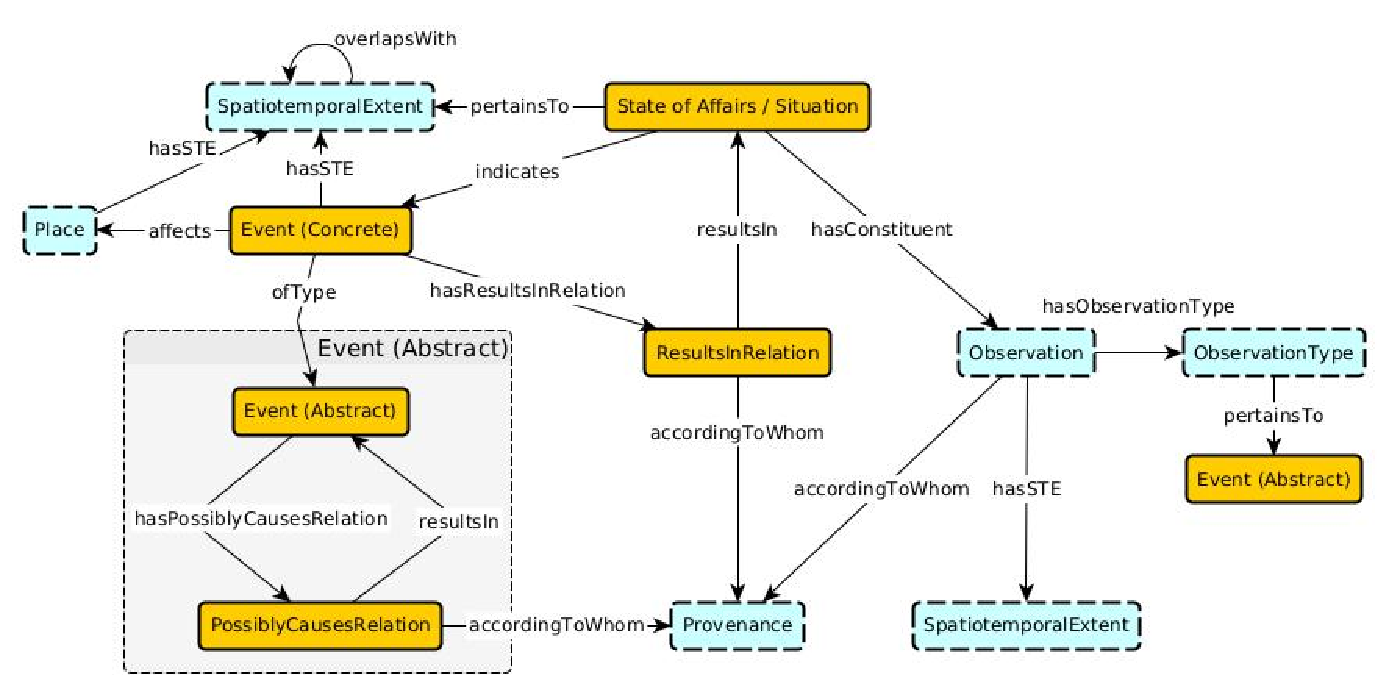
\includegraphics[width=\textwidth]{resources/causal-event-pattern.pdf}
  \end{center}
  \caption{The schema diagram for the Causal Event Pattern.}
  \label{fig:ov-diagram}
\end{figure}


%%%%%%%%%%%%%%%%%%%%%%%%%%%%%%%%%%%
\subsection{Competency Questions}
\label{ssec:cqs}
%%%%%%%%%%
\begin{enumerate}[\phantom{CQ }CQ 1.]
	\item Are there areas in other states than California that are frequently affected by wildfires?
	\item Given fire x, which regions will be effected by smoke exposure, given current wind direction projections?
	\item How were the 2019 Southern California fires affecting the tourism industry?
	\item If I am an agent of an insurance company, what information I can gain from your KWG? (not a competency question, but may help us to think)
	\item Was the Cholera outbreak in Mozambique contributing to the food shortage in year x?
	\item What are the causalities of the wildfire? To answer it, we need spatiotemporal information of temperature, precipitation, soil moisture and etc. in the KG.
	\item What factors can you find in a specific region that would help explain e.g. the stroke belt. Which contaminants of farms may be related from the health literature to strokes?
	\item What farmlands or vegetation covers have been mostly affected in the fire?
	\item What were the reasons for the landslide east of Santa Barbara in April 2017?
	\item What were wildfires affecting the Ventura area in the 2010s?
	\item Where are areas of increased heat exceedance and pollution, where migration is not driven by urbanization?
	\item Where are the places where heat is rising and migration is occurring that cannot be explained by urbanization?
	\item Which farm has High productivity and low connectivity?
	\item Which farm has adopted health soil practice after other nearby farms did so?
	\item Which farm has experienced disease?
	\item Which region affected by a transmissive disease is affected by a hurricane?
	\item Which region affected by the current hurricane just suffers from another natural disaster?
	\item Which regions affected by wildfires are expected to experience heavy rain (flood risk)
	\item Which residents are still evacuated from the same region where the second hurricane hit?
	\item where to deliver Covid-19 supplies?
\end{enumerate}

%%%%%%%%%%%%%%%%%%%%%%%%%%%%%%%%%%%
\subsection{Use Cases}
\label{ssec:use-cases}
%%%%%%%%%%
These are the usecases!

\subsubsection{Direct Relief}
Hurricanes happen in Mozambique; Hurricanes disrupt sewer systems; Cholera is endemic to sub-Saharan region; Mozambique is in Sub-Saharan region; disrupted sewer systems lead to Cholera outbreaks; "this" Hurricane disrupted sewer systems in Mozambique; there were recent outbreaks of Cholera in Mozambique; Mozambique is experiencing a Cholera outbreak due to "this" Hurricane; Cholera outbreaks lead to Vaccination programs

\subsubsection{Thomas Fire}
Thunderstorm in Ventura County results in Wildfire in Ventura County
Wildfire in Ventura County results in low air quality in Santa Barbara
Low air quality in Santa Barbara results in evacuations in Santa Barbara

%%%%%%%%%%%%%%%%%%%%%%%%%%%%%%%%%%%
\subsection{Formalization}
\label{ssec:formalization}
%%%%%%%%%%
\subsubsection{Axioms}
\begin{align}
  \textsf{Place} &\sqsubseteq \forall \textsf{hasSTE.STE} \\
  \exists \textsf{hasSTE.Place} &\sqsubseteq \textsf{STE} \\
  \textsf{Event(Concrete)} &\sqsubseteq \forall \textsf{hasSTE.STE} \\
  \exists \textsf{hasSTE.Event(Concrete)} &\sqsubseteq \textsf{STE} \\
  \textsf{Event(Concrete)} &\sqsubseteq \exists \textsf{hasSTE.Event(Concrete)} \\
  \textsf{Event(Concrete)} &\sqsubseteq \forall \textsf{affects.Place} \\
  \exists \textsf{affects.Event(Concrete)} &\sqsubseteq \textsf{Place} \\
  \textsf{Event(Concrete)} &\sqsubseteq \forall \textsf{ofType.Event(Abstract)} \\
  \exists \textsf{ofType.Event(Concrete)} &\sqsubseteq \textsf{Event(Abstract)} \\
  \textsf{Event(Concrete)} &\sqsubseteq \forall \textsf{hasResultsInRelation.ResultsInRelation} \\
  \exists \textsf{hasResultsInRelation.Event(Concrete)} &\sqsubseteq \textsf{ResultsInRelation} \\
  \textsf{ResultsInRelation} &\sqsubseteq \exists \textsf{hasResultsInRelation}^-\textsf{.ResultsInRelation} \\
  \textsf{STE} &\sqsubseteq \forall \textsf{overlapsWith.STE} \\
  \exists \textsf{overlapsWith.STE} &\sqsubseteq \textsf{STE} \\
  \textsf{StateOfAffairs} &\sqsubseteq \forall \textsf{pertainsTo.STE} \\
  \exists \textsf{pertainsTo.StateOfAffairs} &\sqsubseteq \textsf{STE} \\
  \textsf{StateOfAffairs} &\sqsubseteq \forall \textsf{indicates.Event(Concrete)} \\
  \exists \textsf{indicates.StateOfAffairs} &\sqsubseteq \textsf{Event(Concrete)} \\
  \textsf{StateOfAffairs} &\sqsubseteq \forall \textsf{hasConstituent.Observation} \\
  \exists \textsf{hasConstituent.StateOfAffairs} &\sqsubseteq \textsf{Observation} \\
  \textsf{ResultsInRelation} &\sqsubseteq \forall \textsf{resultsIn.StateOfAffairs} \\
  \exists \textsf{resultsIn.ResultsInRelation} &\sqsubseteq \textsf{StateOfAffairs} \\
  \textsf{ResultsInRelation} &\sqsubseteq \exists \textsf{resultsIn.ResultsInRelation} \\
  \textsf{ResultsInRelation} &\sqsubseteq \forall \textsf{accordingToWhom.Provenance} \\
  \exists \textsf{accordingToWhom.ResultsInRelation} &\sqsubseteq \textsf{Provenance} \\
  \textsf{Observation} &\sqsubseteq \forall \textsf{accordingToWhom.Provenance} \\
  \exists \textsf{accordingToWhom.Observation} &\sqsubseteq \textsf{Provenance} \\
  \textsf{Observation} &\sqsubseteq \forall \textsf{hasSTE.STE} \\
  \exists \textsf{hasSTE.Observation} &\sqsubseteq \textsf{STE} \\
  \textsf{Observation} &\sqsubseteq \forall \textsf{hasObservationType.ObservationType} \\
  \exists \textsf{hasObservationType.Observation} &\sqsubseteq \textsf{ObservationType} \\
  \textsf{ObservationType} &\sqsubseteq \forall \textsf{pertainsTo.Event(Abstract)} \\
  \exists \textsf{pertainsTo.ObservationType} &\sqsubseteq \textsf{Event(Abstract)} \\
  \textsf{Event(Abstract)} &\sqsubseteq \forall \textsf{hasPCR.PCR} \\
  \exists \textsf{hasPCR.Event(Abstract)} &\sqsubseteq \textsf{PCR} \\
  \textsf{PCR} &\sqsubseteq \exists \textsf{hasPCR}^-\textsf{.PCR} \\
  \textsf{PCR} &\sqsubseteq \forall \textsf{resultsIn.Event(Abstract)} \\
  \exists \textsf{resultsIn.PCR} &\sqsubseteq \textsf{Event(Abstract)} \\
  \textsf{PCR} &\sqsubseteq \exists \textsf{resultsIn.PCR} \\
  \textsf{PCR} &\sqsubseteq \forall \textsf{accordingToWhom.Provenance} \\
  \exists \textsf{accordingToWhom.PCR} &\sqsubseteq \textsf{Provenance} \end{align}

\subsubsection{Explanations}
\begin{enumerate}
  \item Scoped Range
  \item Scoped Domain
  \item Scoped Range
  \item Scoped Domain
  \item Existential
  \item Scoped Range
  \item Scoped Domain
  \item Scoped Range
  \item Scoped Domain
  \item Scoped Range
  \item Scoped Domain
  \item Inverse Existential
  \item Scoped Range
  \item Scoped Domain
  \item Scoped Range
  \item Scoped Domain
  \item Scoped Range
  \item Scoped Domain
  \item Scoped Range
  \item Scoped Domain
  \item Scoped Range
  \item Scoped Domain
  \item Existential
  \item Scoped Range
  \item Scoped Domain
  \item Scoped Range
  \item Scoped Domain
  \item Scoped Range
  \item Scoped Domain
  \item Scoped Range
  \item Scoped Domain
  \item Scoped Range
  \item Scoped Domain
  \item Scoped Range
  \item Scoped Domain
  \item Inverse Existential
  \item Scoped Range
  \item Scoped Domain
  \item Existential
  \item Scoped Range
  \item Scoped Domain
\end{enumerate}

%%%%%%%%%%%%%%%%%%%%%%%%%%%%%%%%%%%
\subsection{Submodules}
\label{ssec:submodules}
%%%%%%%%%%
Submodule detection not yet supported.

%%%%%%%%%%%%%%%%%%%%%%%%%%%%%%%%%%%
\subsection{Views}
\label{ssec:views}
%%%%%%%%%%
There are no views documented for this pattern.


%%%%%%%%%%%%%%%%%%%%%%%%%%%%%%%%%%%
\subsection{Entanglements}
\label{ssec:entanglements}
%%%%%%%%%%
There are no entanglements documented for this pattern.

%%%%%%%%%%%%%%%%%%%%%%%%%%%%%%%%%%%
\subsection{Examples}
\label{ssec:examples}
%%%%%%%%%%
\begin{figure}[h!]
  \begin{center}
    \includegraphics[width=\textwidth]{resources/causal-event-example.pdf}
  \end{center}
  \caption{An example ``instantiation'' of the Causal Event Pattern in schema diagram form.}
  \label{fig:ex-diagram}
\end{figure}
\begin{verbatim}
Example Triples
\end{verbatim}

%%%%%%%%%%%%%%%%%%%%%%%%%%%%%%%%%%%
%%%%%%%%%%% End Section %%%%%%%%%%%
%%%%%%%%%%%%%%%%%%%%%%%%%%%%%%%%%%%

%%%%%%%%%%%%%%%%%%%%%%%%%%%%%%%%%%%
\section{Cell Relations Pattern}
\label{sec:cell-relations-pattern}
%%%%%%%%%%%%%%%%%%%%%%%%%%%%%%%%%%%
\subsection{Overview}
\label{ssec:overview}
%%%%%%%%%%
I am the overview.

\begin{figure}[h!]
  \begin{center}
    \includegraphics[width=\textwidth]{resources/cell-relations-pattern.pdf}
  \end{center}
  \caption{The schema diagram for the Cell Relations Pattern.}
  \label{fig:ov-diagram}
\end{figure}


%%%%%%%%%%%%%%%%%%%%%%%%%%%%%%%%%%%
\subsection{Competency Questions}
\label{ssec:cqs}
%%%%%%%%%%
\begin{enumerate}[\phantom{CQ }CQ 1.]
	\item cq1
	\item cq2
\end{enumerate}

%%%%%%%%%%%%%%%%%%%%%%%%%%%%%%%%%%%
\subsection{Use Cases}
\label{ssec:use-cases}
%%%%%%%%%%
These are the usecases!

\subsubsection{Use Case}
Use Case Description

%%%%%%%%%%%%%%%%%%%%%%%%%%%%%%%%%%%
\subsection{Formalization}
\label{ssec:formalization}
%%%%%%%%%%
\subsubsection{Axioms}
\begin{align}
  \textsf{Cell} &\sqsubseteq \forall \textsf{isAdjacentTo.Cell} \\
  \exists \textsf{isAdjacentTo.Cell} &\sqsubseteq \textsf{Cell} \\
  \textsf{Cell} &\sqsubseteq \forall \textsf{contains.Cell} \\
  \exists \textsf{contains.Cell} &\sqsubseteq \textsf{Cell} \\
  \textsf{Cell} &\sqsubseteq \forall \textsf{spatialRelations.Geometry} \\
  \exists \textsf{spatialRelations.Cell} &\sqsubseteq \textsf{Geometry} \\
  \textsf{Cell} &\sqsubseteq \textsf{Geometry} \\
  \textsf{Feature} &\sqsubseteq \forall \textsf{hasGeometry.Geometry} \\
  \exists \textsf{hasGeometry.Feature} &\sqsubseteq \textsf{Geometry} \\
  \textsf{Feature} &\sqsubseteq \exists \textsf{hasGeometry.Feature} \\
  \textsf{Feature} &\sqsubseteq \forall \textsf{hasAttribute.Attribute} \\
  \exists \textsf{hasAttribute.Feature} &\sqsubseteq \textsf{Attribute} \\
  \textsf{Region} &\sqsubseteq \forall \textsf{hasGeometry.Geometry} \\
  \exists \textsf{hasGeometry.Region} &\sqsubseteq \textsf{Geometry} \\
  \textsf{Region} &\sqsubseteq \exists \textsf{hasGeometry.Region} \\
  \textsf{Region} &\sqsubseteq \forall \textsf{hasAttribute.Attribute} \\
  \exists \textsf{hasAttribute.Region} &\sqsubseteq \textsf{Attribute} \\
  \textsf{Attribute} &\sqsubseteq \forall \textsf{hasValue.Quantity} \\
  \exists \textsf{hasValue.Attribute} &\sqsubseteq \textsf{Quantity} \\
  \textsf{Attribute} &\sqsubseteq \exists \textsf{hasValue.Attribute} \\
  \textsf{Attribute} &\sqsubseteq \textsf{Provenance} \end{align}

\subsubsection{Explanations}
\begin{enumerate}
  \item Scoped Range
  \item Scoped Domain
  \item Scoped Range
  \item Scoped Domain
  \item Scoped Range
  \item Scoped Domain
  \item Subclass
  \item Scoped Range
  \item Scoped Domain
  \item Existential
  \item Scoped Range
  \item Scoped Domain
  \item Scoped Range
  \item Scoped Domain
  \item Existential
  \item Scoped Range
  \item Scoped Domain
  \item Scoped Range
  \item Scoped Domain
  \item Existential
  \item Subclass
\end{enumerate}

%%%%%%%%%%%%%%%%%%%%%%%%%%%%%%%%%%%
\subsection{Submodules}
\label{ssec:submodules}
%%%%%%%%%%
Submodule detection not yet supported.

%%%%%%%%%%%%%%%%%%%%%%%%%%%%%%%%%%%
\subsection{Views}
\label{ssec:views}
%%%%%%%%%%
\begin{figure}[h!]
  \begin{center}
    \includegraphics[width=\textwidth]{resources/cell-relations-shortcuts.pdf}
  \end{center}
  \caption{Schema diagram displaying shortcuts for Cell Relations Pattern (red arrows).}
  \label{fig:sc-diagram}
\end{figure}
The shortcuts are as follows.\begin{align}
\textsf{spatiallyRelated}  \circ \textsf{spatialRelations} &\sqsubseteq \textsf{hasGeometry$^-$} \end{align}


%%%%%%%%%%%%%%%%%%%%%%%%%%%%%%%%%%%
\subsection{Entanglements}
\label{ssec:entanglements}
%%%%%%%%%%
There are no entanglements documented for this pattern.

%%%%%%%%%%%%%%%%%%%%%%%%%%%%%%%%%%%
\subsection{Examples}
\label{ssec:examples}
%%%%%%%%%%
There are no examples documented for this pattern.

%%%%%%%%%%%%%%%%%%%%%%%%%%%%%%%%%%%
%%%%%%%%%%% End Section %%%%%%%%%%%
%%%%%%%%%%%%%%%%%%%%%%%%%%%%%%%%%%%

